\chapter{Refactoring}
\section{Code Smells}
\textbf{Code Smell 1 (Long Method):}\\
\lstinputlisting[
	label=code:vorRef,    % Label; genutzt für Referenzen auf dieses Code-Beispiel
	caption=getPlayerAverageOfLeg-Methode vor Refactoring,
	captionpos=b,               % Position, an der die Caption angezeigt wird t(op) oder b(ottom)
	style=EigenerJavaStyle,     % Eigener Style der vor dem Dokument festgelegt wurde
	firstline=1,                
]{Quellcode/getPlayerAverageOfLeg.java}
\lstinputlisting[
	label=code:nachref,    % Label; genutzt für Referenzen auf dieses Code-Beispiel
	caption=getPlayerAverageOfLeg-Methode nach Refactoring,
	captionpos=b,               % Position, an der die Caption angezeigt wird t(op) oder b(ottom)
	style=EigenerJavaStyle,     % Eigener Style der vor dem Dokument festgelegt wurde
	firstline=1,                
]{Quellcode/getPlayerAverageOfLeg_refactored.java}
Die Methode \textit{getPlayerAverageOfLeg} wurde so überarbeitet, dass sie klarer und einfacher zu verstehen ist. Dies wurde durch die Extraktion von Teilen des Codes in separate, private Hilfsmethoden erreicht, die jeweils eine spezifische Aufgabe erfüllen.

Die Methode \textbf{getRoundNumberOfLastRound}: Diese Methode nimmt als Eingabe ein Leg und gibt die Rundennummer der letzten Runde zurück. Sie kapselt den Teil des ursprünglichen Codes, der die Gesamtzahl der Runden ermittelt.

Die Methode \textbf{getSumOfPlayerAveragesOfRounds}: Diese Methode nimmt als Eingabe eine Liste von Round-Objekten und einen Player und gibt die Summe der Durchschnittswerte des Spielers pro Runde zurück. Sie kapselt den Teil des ursprünglichen Codes, der durch die Runden iteriert, um den Durchschnitt des Spielers für jede Runde zu berechnen.

Die Hauptmethode getPlayerAverageOfLeg wurde nun so vereinfacht, dass sie leichter zu verstehen ist. Sie ruft nun einfach die Hilfsmethoden auf und führt eine Berechnung durch, um den Durchschnittswert des Spielers für das Leg zu ermitteln. Dies bietet die Vorteile Wartbarkeit, Lesbarkeit, Testbarkeit und Wiedrverwendbarkeit.\\\\
\textbf{Code Smell 2 (Duplicated Code):}\\
Die Klassen \textit{HandleMatch} und \textit{HandleSet} weisen beide eine Methode auf, die prüft, ob ein Spieler entweder ein komplettes Spiel oder ein Set gewonnen hat. Diese Methoden sind in ihrer Struktur und Logik sehr ähnlich. Der einzige Unterschied besteht darin, dass die Methode in HandleMatch die unterschiedlichen Sets und deren Gewinner berücksichtigt, während die Methode in HandleSet die verschiedenen Legs eines Sets und deren Gewinner in Betracht zieht. Ansonsten sind beide Methoden nahezu identisch. Dies stellt einen deutlichen Fall von doppeltem Code dar, durch dessen Vermeidung etwa 50 Zeilen Code eingespart und die Lesbarkeit, Wiederverwendbarkeit sowie Testbarkeit des Codes verbessert werden könnten.

Zur Lösung dieses Problems mit doppeltem Code wurde die Klasse \textit{HandleGame} eingeführt. Diese Klasse enthält die duplizierten Methoden und dient als Elternklasse für HandleMatch und HandleSet.
\lstinputlisting[
	label=code:ismatchsetwon,    % Label; genutzt für Referenzen auf dieses Code-Beispiel
	caption=Methode isMatchSetWon der Elternklasse,
	captionpos=b,               % Position, an der die Caption angezeigt wird t(op) oder b(ottom)
	style=EigenerJavaStyle,     % Eigener Style der vor dem Dokument festgelegt wurde
	firstline=1,                
]{Quellcode/isMatchSetWon.java}
Die Methode in \autoref{code:ismatchsetwon} wurde wie bereits erwähnt in die Elternklasse HandleGame ausgelagert, womit dieser duplizierte Code gespart wurde.
\lstinputlisting[
	label=code:ismatchsetwonhandleset,    % Label; genutzt für Referenzen auf dieses Code-Beispiel
	caption=Methode isMatchSetWon der HandleSet,
	captionpos=b,               % Position, an der die Caption angezeigt wird t(op) oder b(ottom)
	style=EigenerJavaStyle,     % Eigener Style der vor dem Dokument festgelegt wurde
	firstline=1,                
]{Quellcode/isMatchSetWon_HandleSet.java}
Die Methode in \autoref{code:ismatchsetwonhandleset} ist nun die neue Methode in HandleSet. Die Klasse HandleSet erbt von der Klasse HandleGame, womit die gleiche Funktionalität, wie vor dem Refactoring erreicht wurde.\newpage
\section{2 Refactorings}
\textbf{Refactoring 1 (Extract Method):}\\
Dieses Beispiel bezieht sich auf Commit \href{https://github.com/P3lina/ASE-Project/commit/f50cfec78b045a3a62e5927e44d2699f528aee31}{f50cfec}.\\
\begin{figure}[ht]
    \centering
    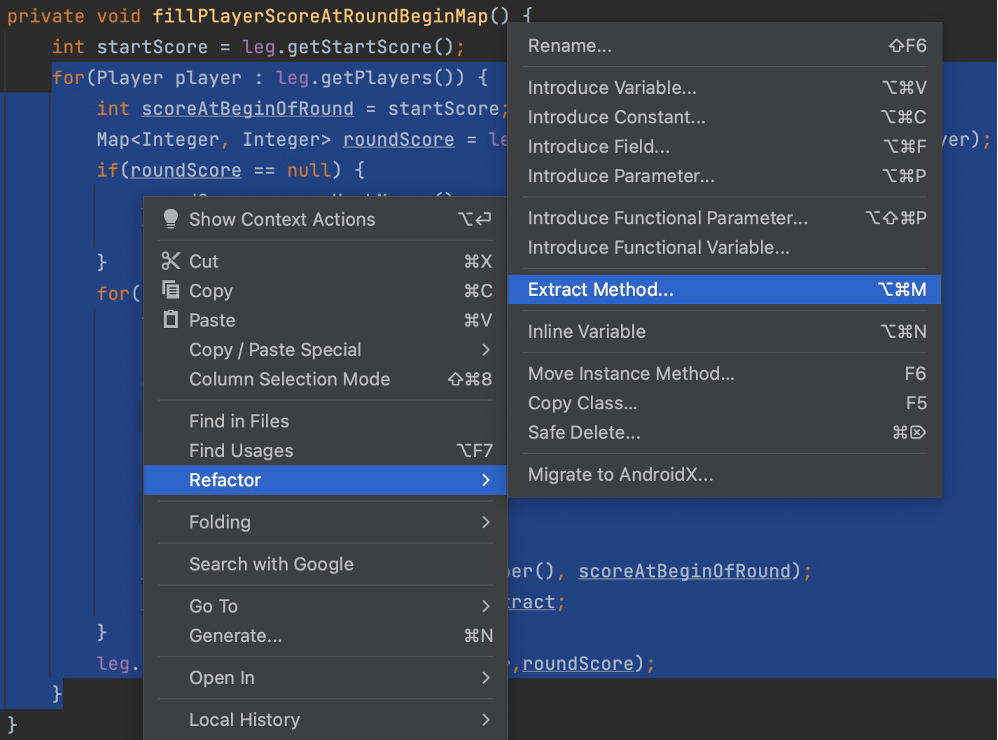
\includegraphics[width=0.6\textwidth]{Bilder/exmeth.png}
    \caption{Extract Method in der \textit{fillPlayerScoreAtRoundBeginMap}-Methode}
    \label{fig:exmeth}
\end{figure}\\
Wie bereits in \autoref{fig:exmeth} in Teilen zu sehen ist, ist die vorgestellte Methode sehr lang und damit unübersichtlich, weswegen sich entschieden wurde, diese Methode in mehrere kleinere, übersichtlichere Methode aufzuteilen.\\
\begin{figure}[ht]
    \centering
    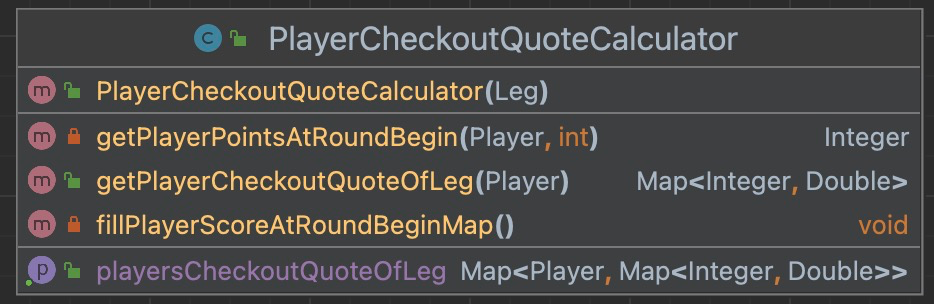
\includegraphics[width=0.6\textwidth]{Bilder/ref1before.png}
    \caption{UML vor Refactor}
    \label{fig:ref1before}
\end{figure}\newpage
\begin{figure}[ht]
    \centering
    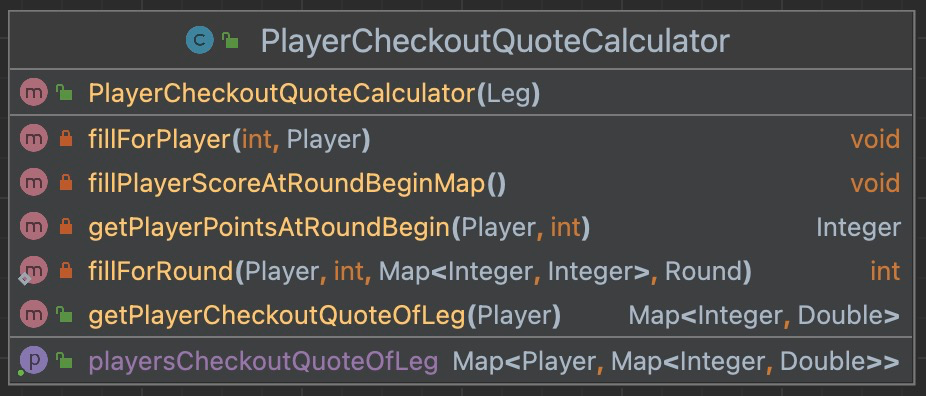
\includegraphics[width=0.6\textwidth]{Bilder/ref1after.png}
    \caption{UML nach Refactor}
    \label{fig:ref1after}
\end{figure}
Wie in \autoref{fig:ref1before} und \autoref{fig:ref1after} zu sehen, wurden 2 neue Methoden hinzugefügt, welche jeweils Verantwortung für einen Teil der ursprünglichen Methode übernehmen. Die Methode \textit{fillPlayerScoreAtRoundBeginMap} ist nun übersichtlicher und leichter zu verstehen.\\\\
\textbf{Refactoring 2 (Replace Conditional with Polymorphism):}\\
Dieses Beispiel bezieht sich auf Commit \href{https://github.com/P3lina/ASE-Project/commit/479ad5e6fddd23eb7df3697e75d55b52b255b301}{479ad5e}\\
\lstinputlisting[
	label=code:prepare,    % Label; genutzt für Referenzen auf dieses Code-Beispiel
	caption=Code vor Refactor,
	captionpos=b,               % Position, an der die Caption angezeigt wird t(op) oder b(ottom)
	style=EigenerJavaStyle,     % Eigener Style der vor dem Dokument festgelegt wurde
	firstline=1,
]{Quellcode/prepareUserDartInput.java}
Wie in \autoref{code:prepare} zu sehen ist, verwendet die Methode 5 if-Statements und einen Default Fall. Dieses if-Statement könnte im Verlauf der Applikation erweitert werden oder es könnten Statements gelöscht oder erweitert werden. Eine hohe Anzahl von if-Zweigen erhöht die Komplexität einer Methode, was das Lesen, Verstehen und Pflegen des Codes erschwert.

Wenn neue Fälle berücksichtigt werden sollen, erfordert dies zusätzliche Arbeit und birgt das Risiko, Fehler zu erzeugen. Zudem kann die Einfügung neuer Bedingungen an irgendeiner Stelle im if-Konstrukt unerwartete Auswirkungen auf die restliche Logik haben.

Zusätzlich kann die Testbarkeit der Methode leiden, da jeder if-Zweig individuell getestet werden muss. Dies erhöht die Anzahl der benötigten Testfälle und die Zeit, die für das Schreiben und Ausführen der Tests benötigt wird.
Deswegen wurde sich entschieden, dieses if-Statement durch Polymorphismus zu ersetzen.\\
\begin{figure}[ht]
    \centering
    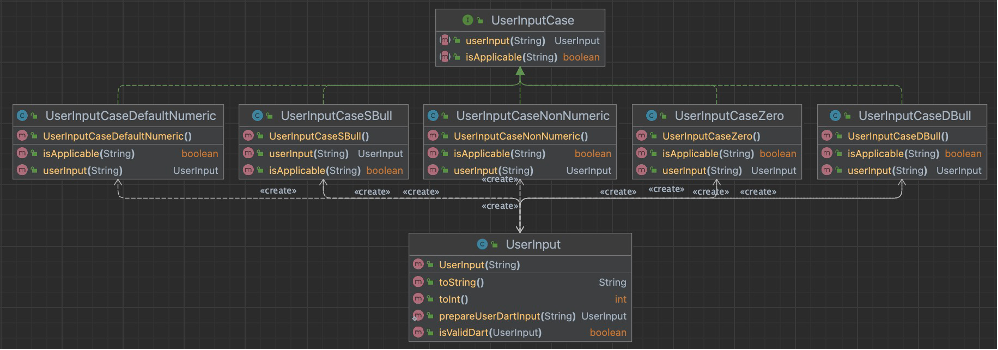
\includegraphics[width=0.9\textwidth]{Bilder/rcwp.png}
    \caption{UML nach Refactor}
    \label{fig:rcwp}
\end{figure}\\
Wie nun in \autoref{fig:rcwp} zu sehen ist, wurden 6 neue Klassen eingeführt. \textit{UserInputCase} ist dabei das Interface, auf dem die anderen Fälle aufbauen und welches die benötigten Methoden für Zutrefflichkeit und Konsens bereitstellt. Diese 5 Klassen implementieren das Interface und überschreiben die Methoden. Die Klasse \textit{UserInputCaseDefault} ist dabei beispielsweise der Default Fall, welcher die Logik des Default Falls aus der ursprünglichen Methode übernimmt.